\chapter{Engineering Analysis}

\section{Thrust Analysis and Drop Requirements}
\label{thrust_analysis}

In order to determine what the required height of the drop was required, the team needed to determine the ability of the rocket to slow down. The goal is for the rocket to touch down on the ground as soft as possible, which would mean the landing velocity would be approaching 0 m/s.

During a drop test, the rocket will be released at a height h, then the sensors with detect a drop, deploy the arms and spin up the rotors. The deployment time will be the time it takes from the drop to the arms being at full thrust. Because of this, we can determine that the initial velocity of the rocket before slow-down would be
\[v_{init} = gt_{deploy}\]
At this time, the momentum of that rocket at that is
\[p_{rocket} = m_{rocket}gt_{deploy}\]
Then, we want to solve for when the rocket is able to return 0 m/s and no longer have any momentum. Looking at a time t, the momentum caused by the impulse from gravity will be
\[p_{gravity} = m_{rocket}gt\]
Further, then at time t, the momentum from the thrust, L, of the rotors will be
\[p_{thrust} = L_{rotors}(t-t_{deploy})\]
Therefore, the at any time t past $t_deploy$, the momentum at that point will be
\[p_{total} = m_{rocket}gt - L_{rotors}(t-t_{deploy})\]
To solve for the t when the total momentum is at 0, we can solve for time t
\[0 = m_{rocket}gt - L_{rotors}(t-t_{deploy})\]
\[L_{rotors}t-L_{rotors}t_{deploy} = m_{rocket}gt\]
\[t(L_{rotors} - m_{rocket}g) = L_{rotors}t_{deploy}\]
\[t = \frac{L_{rotors}t_{deploy}}{(L_{rotors} - m_{rocket}g)}\]
At this time t, the rocket will should hit a hover. 

\noindent Finally, we can get an equation for the distance that the rocket would go through during this time

\[d_{total} = \frac{1}{2}gt_{deploy}^2 + v_{init}(t-t_{deploy}) + \frac{1}{2}(g-L_{rotors})(t-t_{deploy})^2\]
Placing our value in for t
\[d_{total} = \frac{1}{2}gt_{deploy}^2 + v_{init}(\frac{L_{rotors}t_{deploy}}{(L_{rotors} - m_{rocket}g)}-t_{deploy}) + \frac{1}{2}(g-L_{rotors})(\frac{L_{rotors}t_{deploy}}{(L_{rotors} - m_{rocket}g)}-t_{deploy})^2\]
From this, we can solve the equations for multiple different thrust to weight ratios against our weight for different deployment times. This is shown in figure \ref{fig:dvw}

\begin{figure}[H]
    \centering
    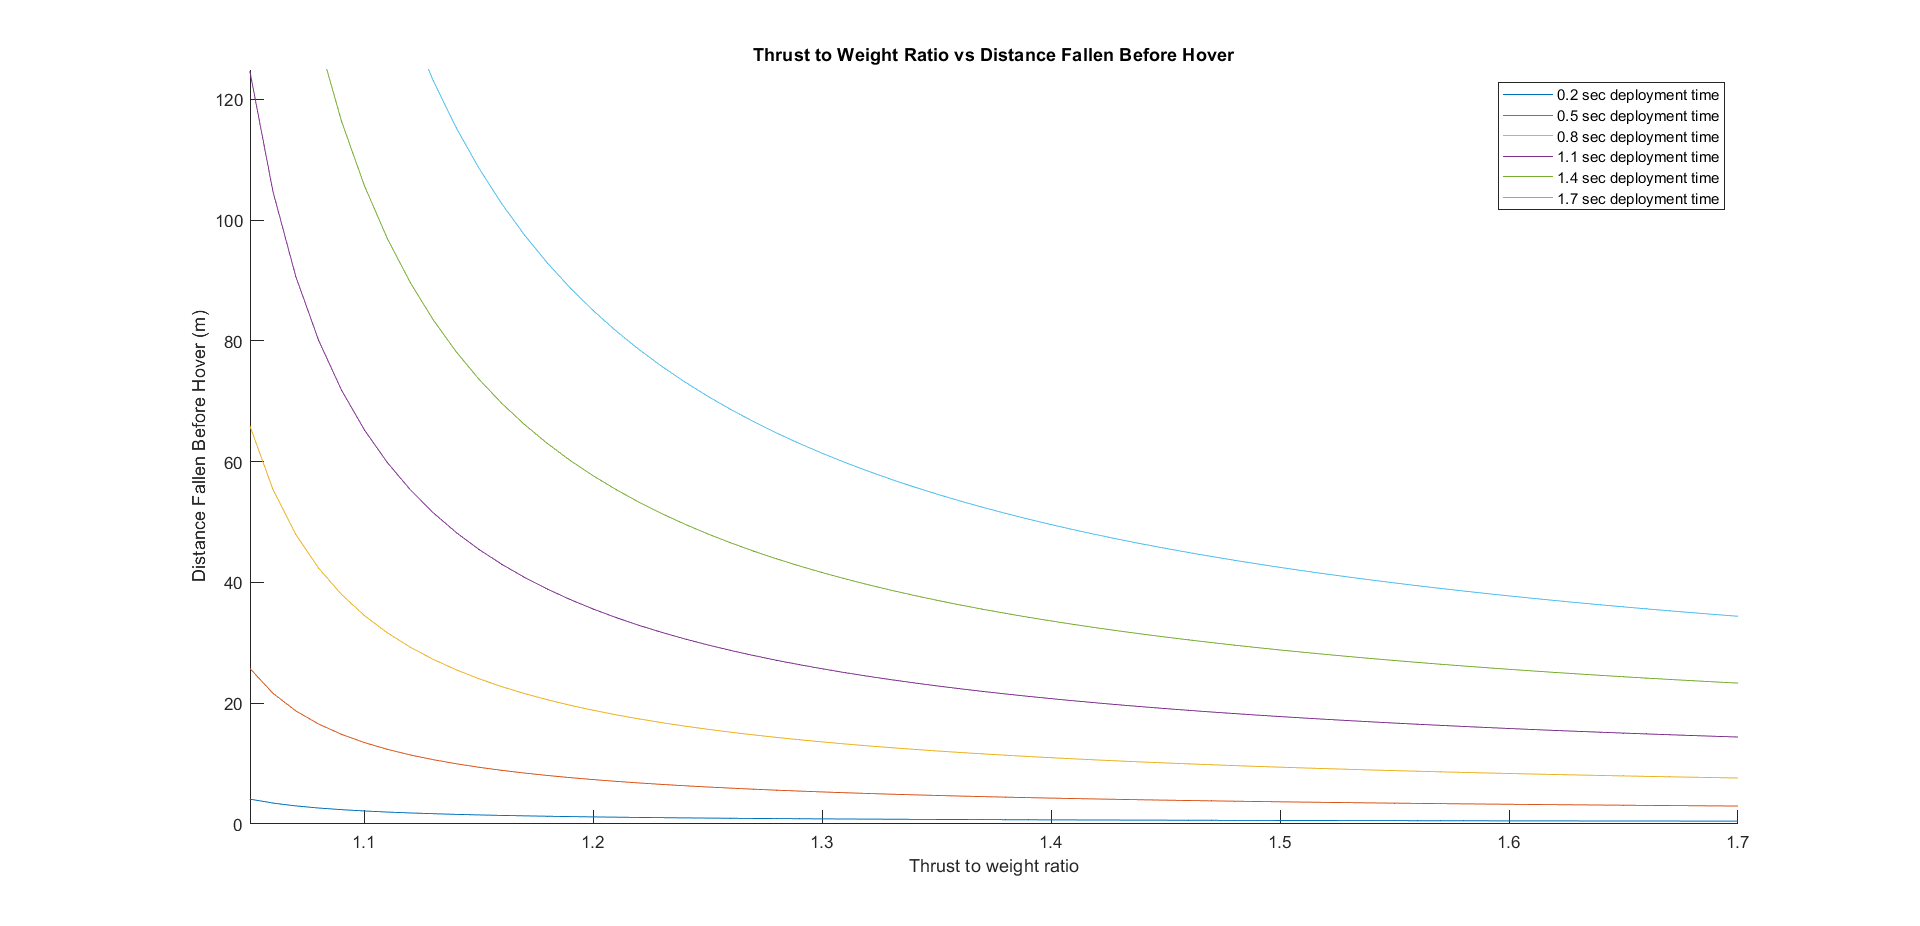
\includegraphics[width=\textwidth]{src/figs/ThrusttoWeight_Distance.png}
    \caption{Distance fallen versus thrust to weight ratio}
    \label{fig:dvw}
\end{figure}

From this we can see that making the thrust to weight ratio as high as possible is very important along with minimizing the deployment time. With our rocket's mass at 3.25 kg, the thrust at 10 N and the deployment time at 0.8 seconds, we would need 15.68 m of drop height. 

\section{Center of Mass Analysis}
In a drone body, it is ideal to have the center of mass of the at the same height as the blades (i.e. the center of thrust), in order for torque from the arms to be able to rotate the body easier. Because of this, we wanted to design a rocket body with a center of mass close approaching this value. In our design method, we programmed an excel sheet to took into account the mass of each component along with its distance from the top of the rocket. Then, it finds moment of each of the components along each axis. Dividing that value by the mass gives us the center of mass as a distance from the top of the rocket. The code was tested against an experimental result and was accurate within a quarter of an inch.

This is important because it allows for the the team to decide on how to change the location of components and how those decisions change the COM. This was used during mass optimization steps. The final result was the COM being 8.1 inches below the blades in their deployed position.



\section{Structural Analysis of Parts}
In order to determine whether or not the designed components would be able to withstand the loads imposed on them by the deployment torsion springs and the thrust from the motors, several ANSYS Static Structural Simulations were performed throughout the quarter. The simulations for the alpha prototype components can be found below.


\subsection{Propulsion Arm}
\label{propulsionarmansys}
The propulsion arm is subject to two loading conditions. The first of which is in the stowed position. One end of the arm has a torque imposed by the torsion springs totaling 0.6 Nm at 90 degrees of spring deflection. The other end of the arm interfaces with the pre-deployment locking disk. To model this in ANSYS, a torque of 0.8 Nm was applied around the axle support mounts. Additionally, a fixed support was added on the disk interface as well as the axle mounts. The arm material was set to 6060 T6 Aluminum since MarkForged advertises their Carbon Fiber reinforced Onyx as similar in strength to this. Monitors for deformation and equivalent stress were added and the solution was ran. The resulting contour plots can be seen below in \ref{fig:stowedarmdef} and \ref{fig:stowedarmstress}, respectively. From these, it can be seen that the maximum deformation is 2.45e-6 m and the maximum equivalent stress is 1.84e6 Pa, well within the material limits of the Onyx CF print.
\begin{figure}[H]
    \centering
    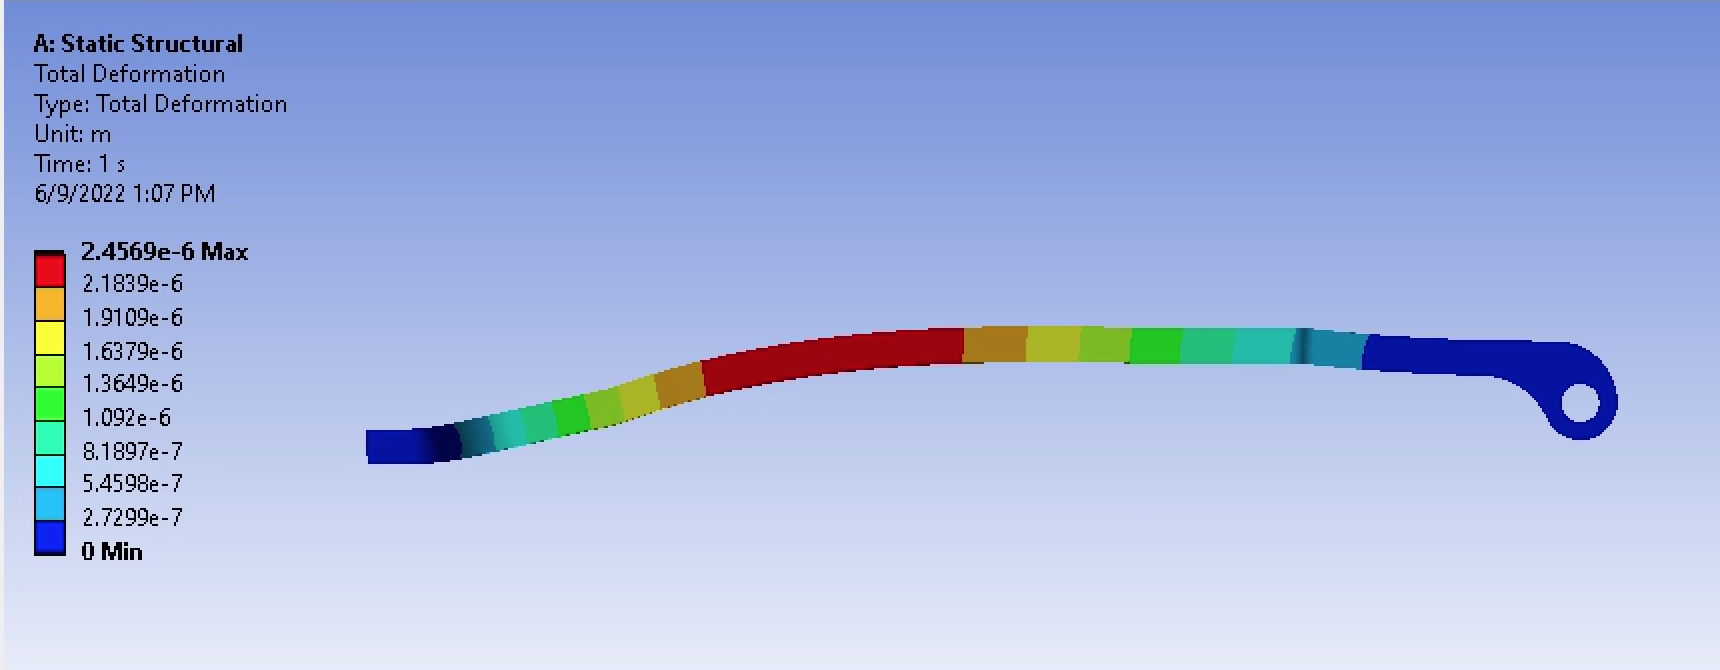
\includegraphics[width=\textwidth]{src/figs/stowed-arm-def.png}
    \caption{Stowed Propulsion Arm Deformations}
    \label{fig:stowedarmdef}
\end{figure}
\begin{figure}[H]
    \centering
    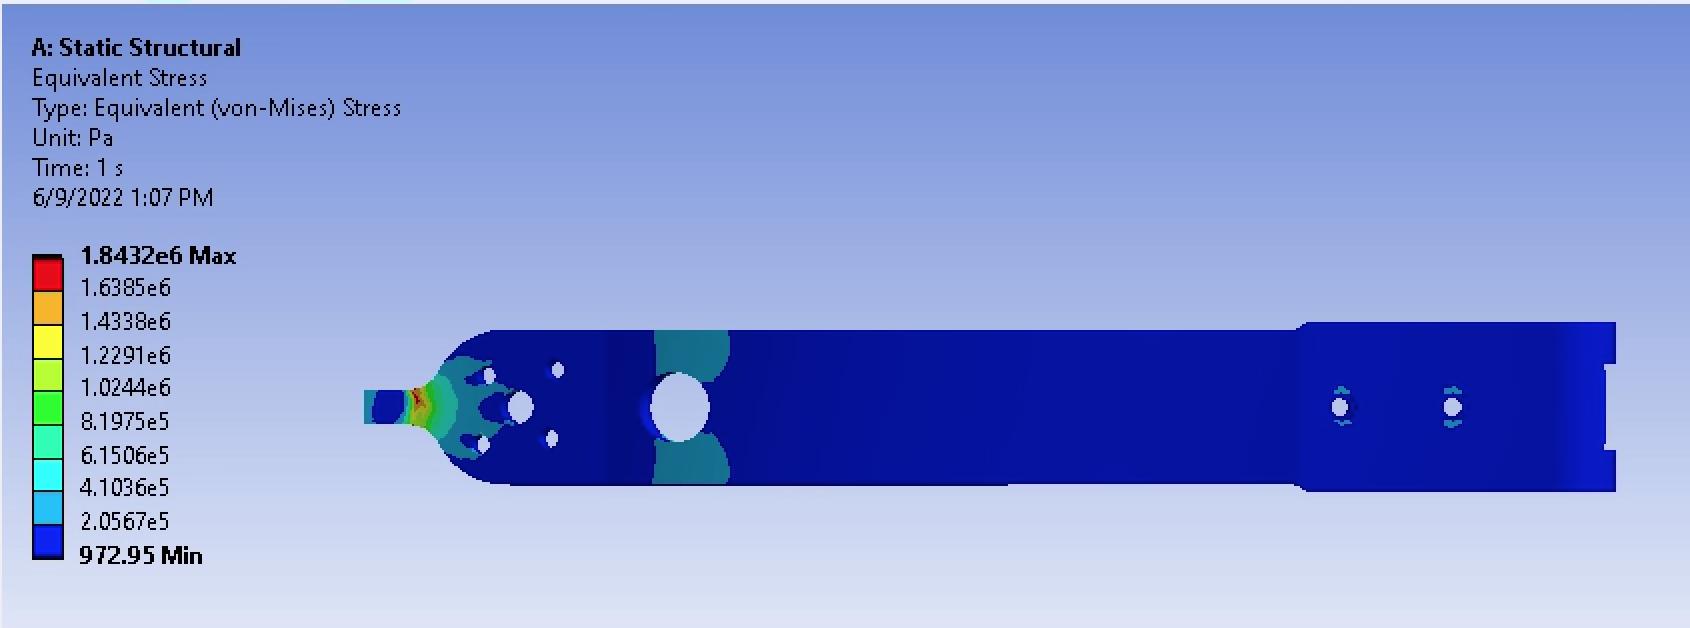
\includegraphics[width=\textwidth]{src/figs/stowed-arm-stress.png}
    \caption{Stowed Propulsion Arm Stress}
    \label{fig:stowedarmstress}
\end{figure}

The other loading condition the arm will sustain is in its deployed position with thrust applied. To model this, the fixed supports were kept on the axle support and one was added on the interface with the core. The disk interface support was removed. A thrust force of 15N (a 1.5 FOS from our expected max thrust) was applied at the motor mount. Monitors for deformation and equivalent stress were added and the simulation was ran. The contour plots for the deformation and stress can be seen below in figures \ref{fig:deployedarmdef} and \ref{fig:deployedarmstress}, respectively. From these plots the maximum deformation is 0.4 mm and the maximum equivalent stress is 18.258 MPa, well within the limits of the Onyx CF. 
\begin{figure}[H]
    \centering
    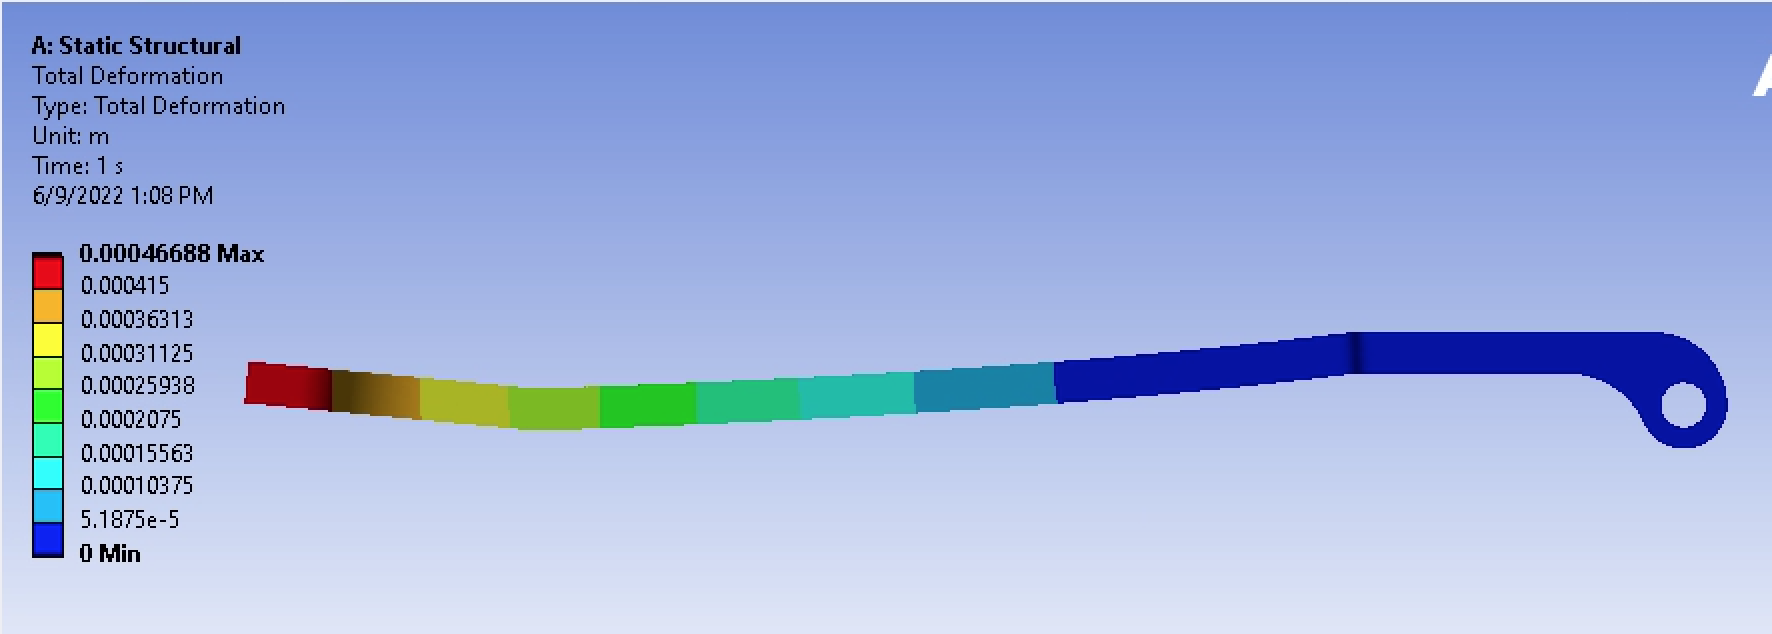
\includegraphics[width=\textwidth]{src/figs/deployed-arm-def.png}
    \caption{Deployed Arm Deformation}
    \label{fig:deployedarmdef}
\end{figure}
\begin{figure}[H]
    \centering
    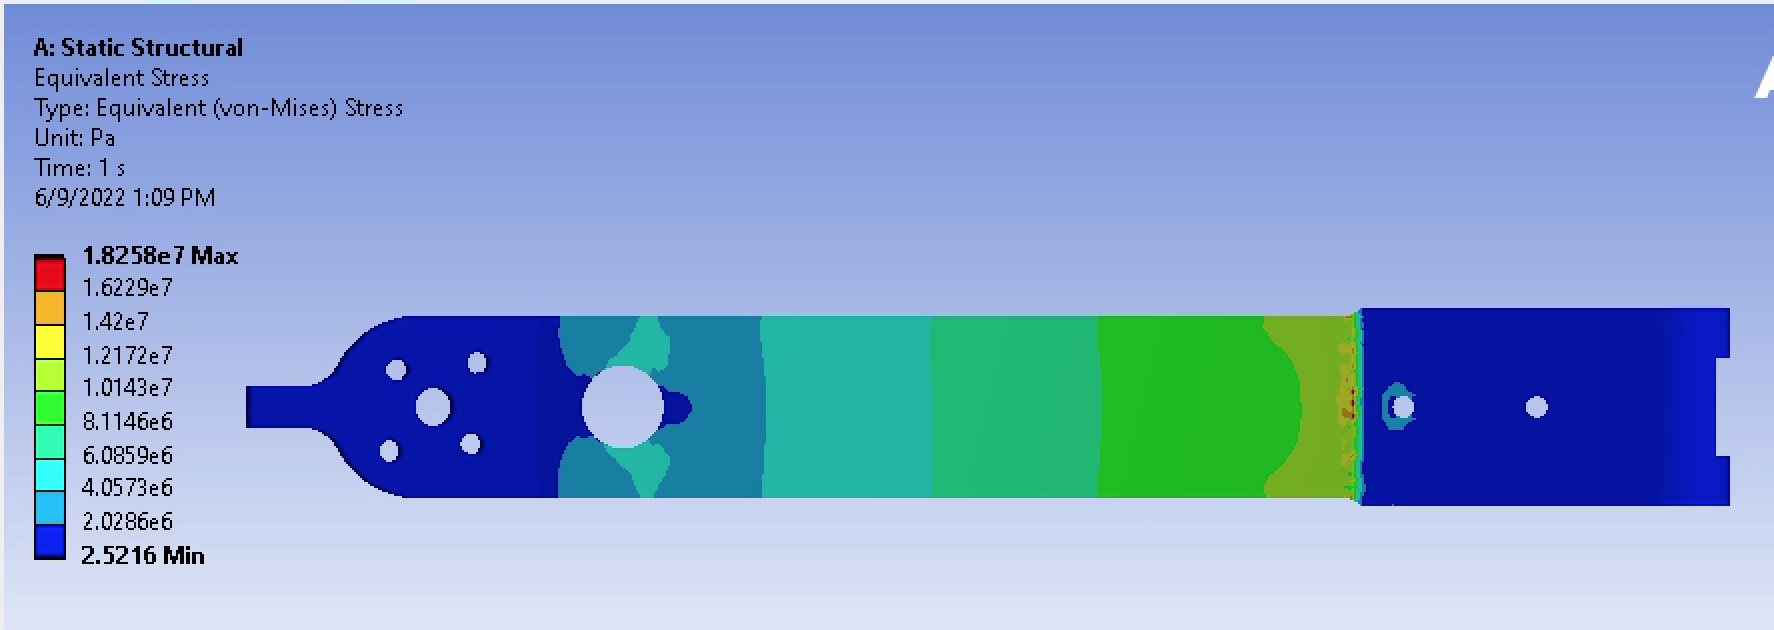
\includegraphics[width=\textwidth]{src/figs/deployed-arm-stress.png}
    \caption{Deployed Arm Stress}
    \label{fig:deployedarmstress}
\end{figure}

\subsection{Core}
An analysis was done with our previous core but not fulfilled in the Alpha core. Since the cores are very similar structures, with the forces going in the same direction, and since we did not observe any notable deformation in the new design during physical testing, we believe that our results for the old core will be similar in the new setup and our results are relevant.


The core will also be taking a substantial load since the propulsion arm will be pushing against it when full thrust is applied. To ensure that the core will not yield under these loads, it too was modeled in ANSYS static structural. To do this, fixed supports were added where it mounts to the threaded rods. The arms were modeled with the core and constrained so that they were in contact with the top surface of the core. The thrust force with a 1.5 FOS was added to the ends of the arm and total deformation and equivalent stress was plotted. These plots can be seen below in figures \ref{fig:CoreDef} and \ref{fig:CoreDef2}. From these plots it can be seen that the maximum deformation is 0.3 mm and the maximum equivalent stress is 917.51 psi, within the limits of the ABS print material properties. 

\begin{figure}[H]
    \centering
    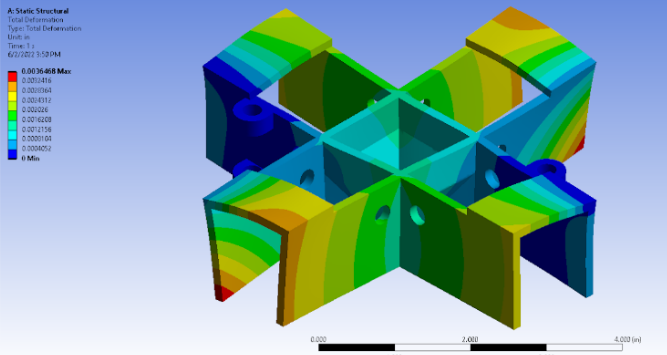
\includegraphics[width=\textwidth]{src/figs/CoreAnsys.png}
    \caption{Deformation of Core from Forces}
    \label{fig:CoreDef}
\end{figure}

\begin{figure}[H]
    \centering
    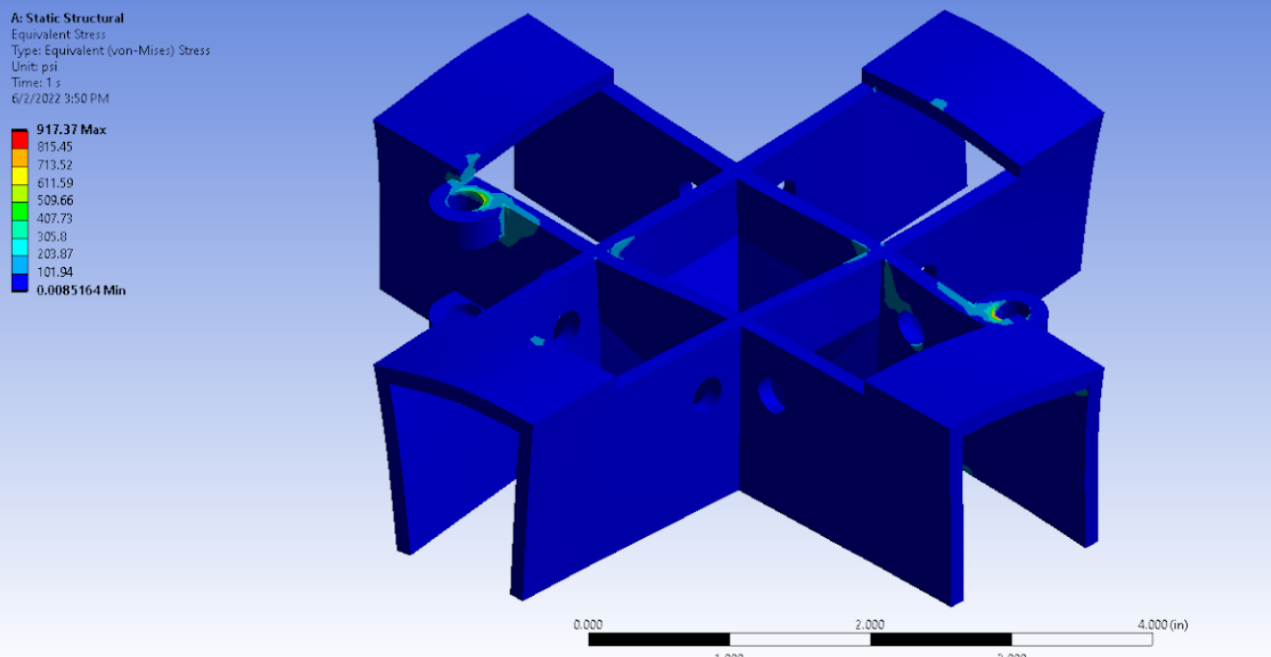
\includegraphics[width=0.9\textwidth]{src/figs/CoreAnsys2.png}
    \caption{Stress of Core from Forces}
    \label{fig:CoreDef2}
\end{figure}


\subsection{Pre-Deployment Locking Disk}
The pre-deployment locking disk will also undergo minor loading when the arm is in the stowed position. To model this, a fixed support was added where the disk interfaces with the leg unlocking spool. Additionally, a force of 4.2 N was added to each tab, equivalent of the torque from both torsion springs at 7.5 inches from the spring. Monitors were added for deformation and equivalent stress and the simulation was run. These plots can be seen in Figure \ref{fig:diskdef} and Figure \ref{fig:diskstress}. From these, the maximum deformation and maximum equivalent stress are 0.0000043 meters and 0.55 MPa respectively, within the limits of the ABS print.
\begin{figure}[H]
    \centering
    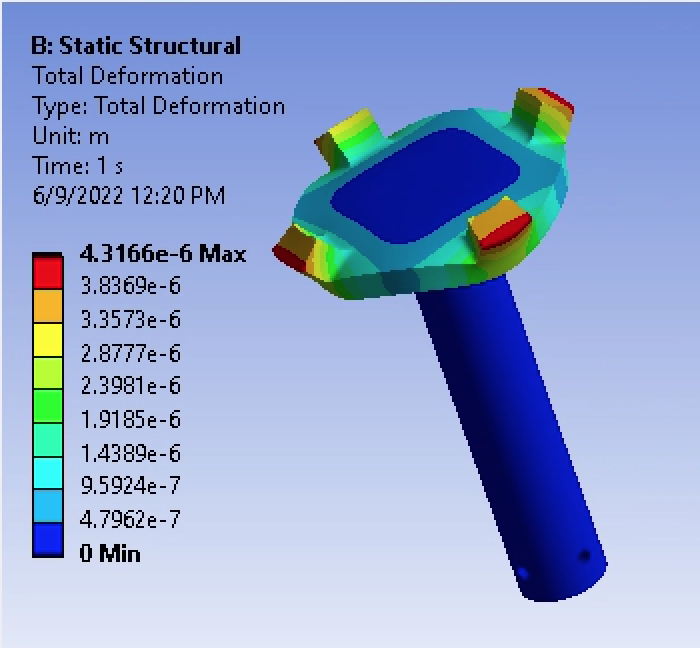
\includegraphics[width=0.9\textwidth]{src/figs/disk-deformation.png}
    \caption{Pre-Deployment Locking Disk Total Deformation}
    \label{fig:diskdef}
\end{figure}
\begin{figure}[H]
    \centering
    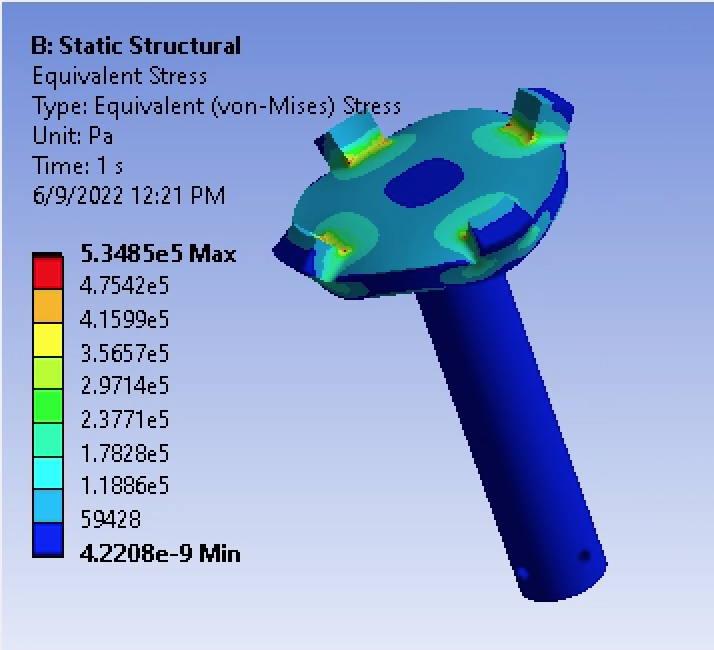
\includegraphics[width=0.9\textwidth]{src/figs/disk-stress.png}
    \caption{Pre-Deployment Locking Disk Equivalent Stress}
    \label{fig:diskstress}
\end{figure}


